\documentclass[12pt,a4paper]{article}
\usepackage{courier}
\usepackage{nopageno}
\usepackage[polish]{babel}
\usepackage[T1]{fontenc}
\usepackage[utf8]{inputenc}
\usepackage{amsmath,amsfonts}
\usepackage{titling}
\usepackage{mathtools}
\usepackage[margin=0.6in]{geometry} 
\usepackage{enumerate}
\usepackage{graphicx}

\title{Ćwiczenia z Sieci komputerowych \\ Lista 1 -- Rozwiązania}
\author{Cezary Świtała}

\begin{document}

\maketitle

\vskip 0.2cm
\noindent
\textbf{Deklaruję zadania: 1, 2, 3, 4, 5, 6, 7, 9, 10}
\vskip 0.2cm


\noindent
\textbf{Zadanie 1} Dla każdego z podanych poniżej adresów IP w notacji CIDR określ, czy jest to adres sieci, adres rozgłoszeniowy czy też adres komputera. W każdym przypadku wyznacz odpowiadający mu adres sieci, i jakiś adres IP innego komputera w tej samej sieci.
\vskip 0.2cm

\noindent
\textbf{Rozwiązanie:}
\begin{itemize}
	\item \texttt{10.1.2.3/8} -- adres komputera \\ 
		Adres sieci: \texttt{10.0.0.0/8} \\
		Adres rozgłoszeniowy: \texttt{10.255.255.255/8} \\
		Adres innego komputera: \texttt{10.0.0.1/8}
	\item \texttt{156.17.0.0/16} -- adres sieci \\
		Adres rozgłoszeniowy: \texttt{156.17.255.255/16} \\
		Adres przykładowego komputera: \texttt{156.17.0.1/16}
	\item \texttt{99.99.99.99/27} -- adres komputera \\
		Adres sieci: \texttt{99.99.99.96/27} \\
		Adres rozgłoszeniowy: \texttt{99.99.99.127/27}
	\item \texttt{156.17.64.4/30} -- adres sieci \\
		Adres rozgłoszeniowy: \texttt{156.17.64.7/30} \\
		Adres komputera: \texttt{156.17.64.5/30}
	\item \texttt{123.123.123.123/32} -- adres jedynego komputera w sieci o takim samym adresie.
\end{itemize}

\vskip 0.2cm
\noindent
\textbf{Zadanie 2} Podziel sieć \texttt{10.10.0.0/16} na 5 rozłącznych podsieci, tak aby każdy z adresów IP sieci \texttt{10.10.0.0/16} był w jednej z podsieci. Jak zmieniła się liczba adresów IP możliwych do użycia przy adresowaniu komputerów? Jaki jest minimalny rozmiar podsieci, który możesz uzyskać w ten sposób.
\vskip 0.2cm

\noindent
\textbf{Rozwiązanie:}
Najpierw dzielimy sieć na 2 równe części. Powstałe połówki po raz kolejny dzielimy na pół. Następnie wybieramy jedną z powstałych sieci i dzielimy ją na pół. Powstaną w ten sposób następujące sieci:

\begin{itemize}
	\item \texttt{10.10.64.0/18}
	\item \texttt{10.10.128.0/18}
	\item \texttt{10.10.192.0/18}
	\item \texttt{10.10.0.0/19}
	\item \texttt{10.10.32.0/19}
\end{itemize}

\noindent
Sytuację tą obrazuje poniższe drzewo:
\begin{center}
	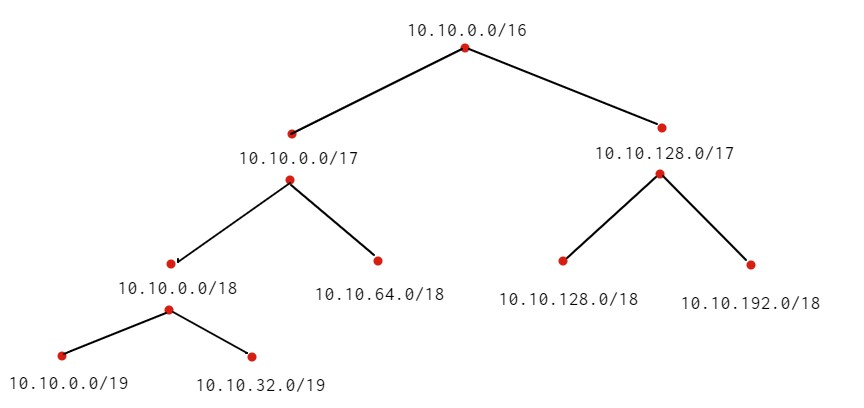
\includegraphics[scale=0.6]{tree}
\end{center}


\noindent
Każdy adres z puli sieci \texttt{10.10.0.0/16} należy do jednej z powyższych, gdyż powstały one przez podział sieci początkowej.

Liczba dostępnych adresów IP zmniejszy się, gdyż na każdą podsieć potrzebujemy zarezerwować jej adres oraz adres rozgłoszeniowy, czyli 10 adresów. Sieć \texttt{10.10.0.0/16} wcześniej również potrzebowała tego typu adresów, zatem liczba zmarnowanych adresów zwiększyła się tylko o 8.

Żeby znaleźć minimalny rozmiar sieci, którą da się utworzyć w ten sposób musimy spróbować zmaksymalizować wysokość takiego drzewa jak powyżej (czyli, w którym schodzimy 1 bit maski na raz). Przykład takiego najwyższego drzewa:

\begin{center}
	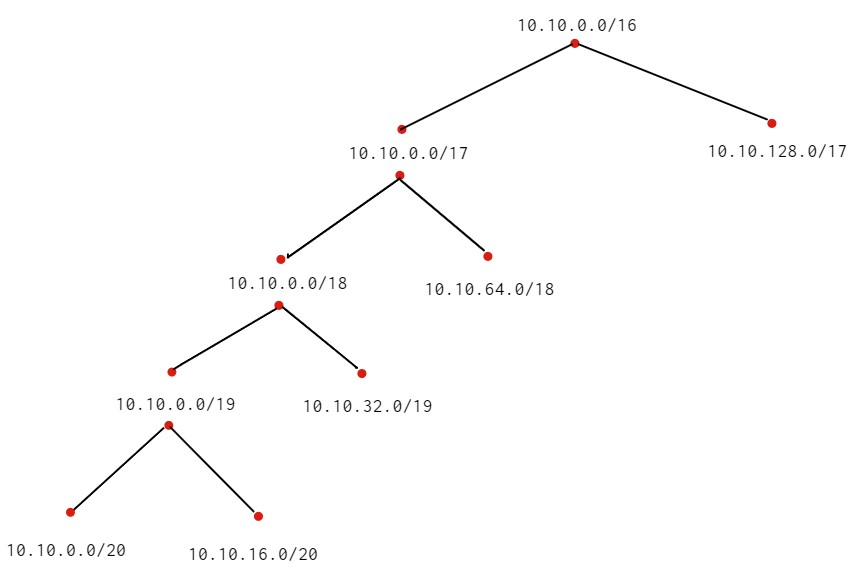
\includegraphics[scale=0.6]{tree2}	
\end{center}

\noindent
Zauważmy, że nie da się utworzyć wyższego drzewa, gdyż są to pełne drzewa binarne (czyli każdy wierzchołek ma 0 albo 2 dzieci), więc jeśli wysokość byłaby większa, to oznaczałoby to, że mamy co najmniej 5 rozgałęzień po drodze od korzenia do najgłębszego liścia, a co za tym idzie -- co najmniej 6 liści, gdyż każde rozgałęzienie oznacza nowego liścia (no i wliczamy początkowy korzeń).

Zatem sieci znajdujące się na głębokości 4 to najmniejsze jakie jesteśmy w stanie uzyskać, a ich rozmiar to \( 2^{12} - 2 = 4094 \).

\newpage
\noindent
\textbf{Zadanie 3} Tablica routingu zawiera następujące wpisy (podsieć \(\rightarrow\) dokąd wysłać):

\begin{itemize}
	\item \texttt{0.0.0.0/0} \(\rightarrow\) do routera \(A\).
	\item \texttt{10.0.0.0/23} \(\rightarrow\) do routera \(B\).
	\item \texttt{10.0.2.0/24} \(\rightarrow\) do routera \(B\).
	\item \texttt{10.0.3.0/24} \(\rightarrow\) do routera \(B\).
	\item \texttt{10.0.1.0/24} \(\rightarrow\) do routera \(C\).
	\item \texttt{10.0.0.128/25} \(\rightarrow\) do routera \(B\).
	\item \texttt{10.0.1.8/29} \(\rightarrow\) do routera \(B\).
	\item \texttt{10.0.1.16/29} \(\rightarrow\) do routera \(B\).
	\item \texttt{10.0.1.24/29} \(\rightarrow\) do routera \(B\).
\end{itemize}

Napisz równoważną tablicę routingu zawierającą jak najmniej wpisów.
\vskip 0.2cm

\noindent
\textbf{Rozwiązanie:} Narysujmy wykres analogiczny do tych z wykładu:

\begin{center}
	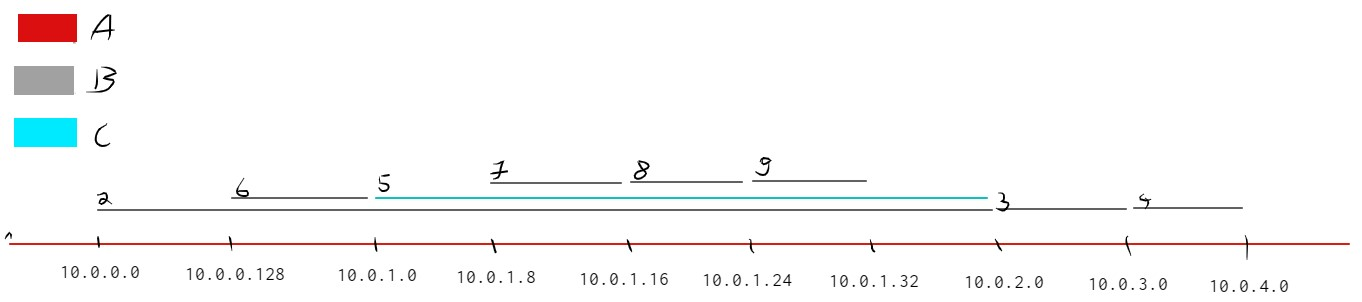
\includegraphics[scale=0.5]{z3prz}	
\end{center}

Po zminimalizowaniu:

\begin{center}
	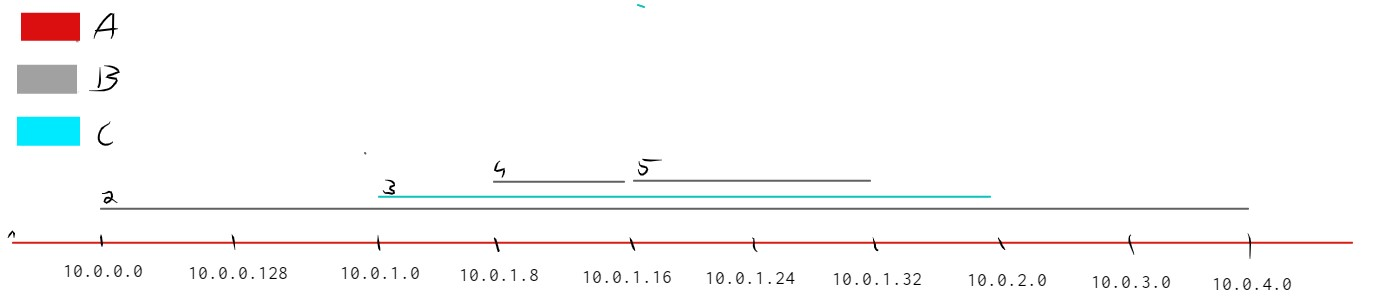
\includegraphics[scale=0.5]{z3po}	
\end{center}

\begin{itemize}
	\item \texttt{0.0.0.0/0} \(\rightarrow\) do routera \(A\).
	\item \texttt{10.0.0.0/22} \(\rightarrow\) do routera \(B\).
	\item \texttt{10.0.1.0/24} \(\rightarrow\) do routera \(C\).
	\item \texttt{10.0.1.8/29} \(\rightarrow\) do routera \(B\).
	\item \texttt{10.0.1.16/28} \(\rightarrow\) do routera \(B\).
\end{itemize}

\newpage
\noindent
\textbf{Zadanie 4} Wykonaj powyższe zadanie dla tablicy:

\begin{itemize}
	\item \texttt{0.0.0.0/0} \(\rightarrow\) do routera \(A\).
	\item \texttt{10.0.0.0/8} \(\rightarrow\) do routera \(B\).
	\item \texttt{10.3.0.0/24} \(\rightarrow\) do routera \(C\).
	\item \texttt{10.3.0.32/27} \(\rightarrow\) do routera \(B\).
	\item \texttt{10.3.0.64/27} \(\rightarrow\) do routera \(B\).
	\item \texttt{10.3.0.96/27} \(\rightarrow\) do routera \(B\).
\end{itemize}

\vskip 0.2cm

\noindent
\textbf{Rozwiązanie:} Narysujmy wykres analogiczny do tych z wykładu:

\begin{center}
	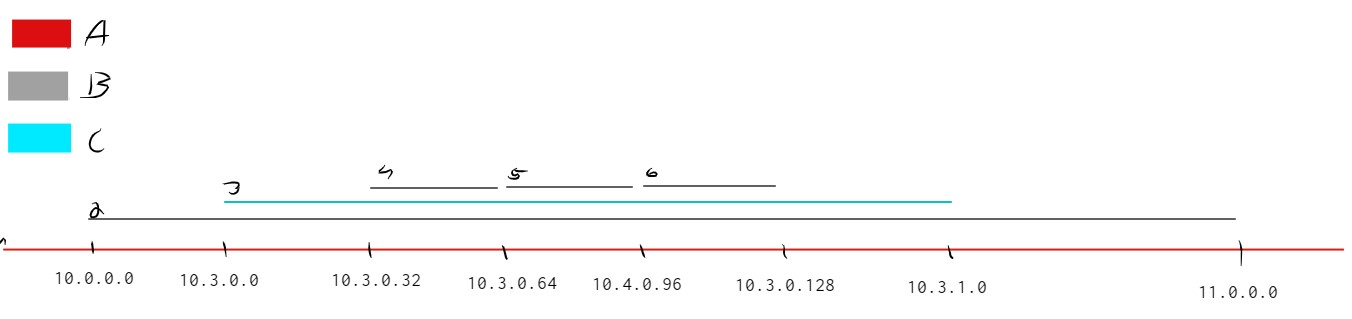
\includegraphics[scale=0.5]{z4prz}	
\end{center}

Po zminimalizowaniu:

\begin{center}
	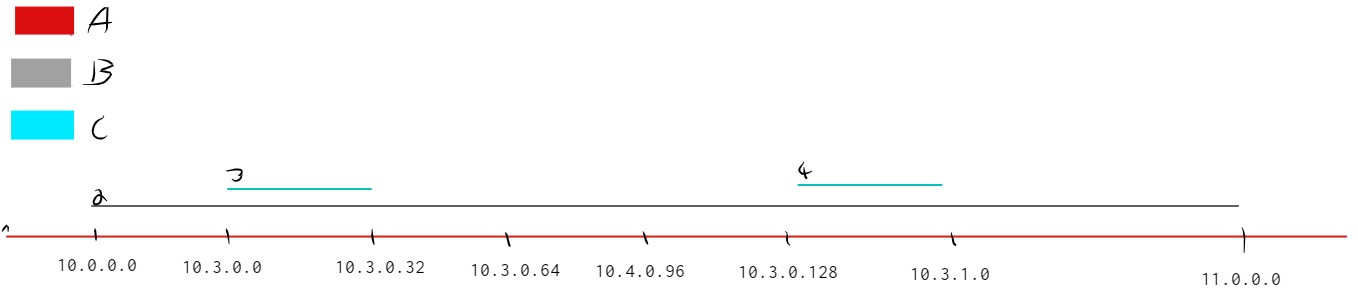
\includegraphics[scale=0.5]{z4po}	
\end{center}

\begin{itemize}
	\item \texttt{0.0.0.0/0} \(\rightarrow\) do routera \(A\).
	\item \texttt{10.0.0.0/8} \(\rightarrow\) do routera \(B\).
	\item \texttt{10.3.0.0/27} \(\rightarrow\) do routera \(C\).
	\item \texttt{10.3.0.128/25} \(\rightarrow\) do routera \(C\).
\end{itemize}

\vskip 0.2cm
\noindent
\textbf{Zadanie 5} Jak uporządkować wpisy w tablicy routingu, żeby zasada najlepszego dopasowania odpowiadała wyborowi ,,pierwszy pasujący'' (tj. przeglądaniu tablicy od początku do końca aż do momentu napotkania dowolnej pasującej reguły)? Odpowiedź uzasadnij formalnie.
\vskip 0.2cm

\noindent
\textbf{Rozwiązanie:} Wpisy tablicy sortujemy nierosnąco względem długości maski (prefiksu).
\vskip 0.2cm

\noindent
\textbf{Uzasadnienie:} Niech \(x\) będzie adresem, dla którego szukamy najdłuższego dopasowania prefiksu, a \(x'\) pierwszym adresem, który się do niego dopasował w trakcie przeglądania posortowanej tablicy. Załóżmy nie wprost, że istnieje inny wpis \(y\), który posiada dłuższy wspólny prefiks z \(x\). Skoro jeszcze go nie przejrzeliśmy, to długość jego maski jest mniejsza lub równa tej z \(x'\). Ponieważ oba adresy dopasowują się do \(x\), to \(y\) jest prefiksem \(x'\), zatem nie może posiadać większego wspólnego prefiksu z \(x\). Sprzeczność.

\vskip 0.2cm
\noindent
\textbf{Zadanie 6} W podanej niżej sieci, tablice routingu budowane są za pomocą algorytmu wektora odległości. Pokaż (krok po kroku), jak będzie się to odbywać. W ilu krokach zostanie osiągnięty stan stabilny?
\vskip 0.2cm

\noindent
\textbf{Rozwiązanie:} Zaczynamy od stanu, w którym każda maszyna jest świadoma swojego bezpośredniego sąsiedztwa i wykonujemy kroki protokołu.

\vskip 0.2cm
\begin{tabular}{ | c | c | c | c | c | c | c | }
 \hline
      & A & B & C & D & E & F \\
 \hline
 do A & - & 1 &   &   &   &   \\
 do B & 1 & - & 1 &   &   &   \\
 do C &   & 1 & - &   & 1 & 1 \\
 do D &   &   &   & - & 1 &   \\
 do E &   &   & 1 & 1 & - & 1 \\
 do F &   &   & 1 &   & 1 & - \\
 do S & 1 & 1 &   &   &   &   \\
 \hline
\end{tabular}

\vskip 0.2cm
\begin{tabular}{ | c | c | c | c | c | c | c | }
 \hline
      &     A   &     B    &    C    &    D    &     E   &    F    \\
 \hline
 do A & -       & 1        & 2 via B &         &         &         \\
 do B & 1       & -        & 1       &         & 2 via C & 2 via C \\
 do C & 2 via B & 1        & -       & 2 via E & 1       & 1       \\
 do D &         &          & 2 via E & -       & 1       & 2 via E \\
 do E &         & 2 via C  & 1       & 1       & -       & 1       \\
 do F &         & 2 via C  & 1       & 2 via E & 1       & -       \\
 do S & 1       & 1        & 2 via B &         &         &         \\
 \hline
\end{tabular}

\vskip 0.2cm
\begin{tabular}{ | c | c | c | c | c | c | c | }
 \hline
      &     A   &     B    &    C    &    D    &     E   &    F    \\
 \hline
 do A & -       & 1        & 2 via B &         & 3 via C & 3 via C \\
 do B & 1       & -        & 1       & 3 via E & 2 via C & 2 via C \\
 do C & 2 via B & 1        & -       & 2 via E & 1       & 1       \\
 do D &         & 3 via C  & 2 via E & -       & 1       & 2 via E \\
 do E & 3 via B & 2 via C  & 1       & 1       & -       & 1       \\
 do F & 3 via B & 2 via C  & 1       & 2 via E & 1       & -       \\
 do S & 1       & 1        & 2 via B &         & 3 via C & 3 via C \\
 \hline
\end{tabular}

\vskip 0.2cm
\begin{tabular}{ | c | c | c | c | c | c | c | }
 \hline
      &     A   &     B    &    C    &    D    &     E   &    F    \\
 \hline
 do A & -       & 1        & 2 via B & 4 via E & 3 via C & 3 via C \\
 do B & 1       & -        & 1       & 3 via E & 2 via C & 2 via C \\
 do C & 2 via B & 1        & -       & 2 via E & 1       & 1       \\
 do D & 4 via B & 3 via C  & 2 via E & -       & 1       & 2 via E \\
 do E & 3 via B & 2 via C  & 1       & 1       & -       & 1       \\
 do F & 3 via B & 2 via C  & 1       & 2 via E & 1       & -       \\
 do S & 1       & 1        & 2 via B & 4 via E & 3 via C & 3 via C \\
 \hline
\end{tabular}

\vskip 0.2cm
Po trzech krokach wektory znalazły się w stanie stabilnym.

\newpage
\noindent
\textbf{Zadanie 7} Załóżmy, że w powyższej sieci tablice routingu zostały już zbudowane. Co będzie się działo, jeśli dodane zostanie połączenie między routerami \(A\) i \(D\).
\vskip 0.2cm

\noindent
\textbf{Rozwiązanie:} Routery \(A\) i \(D\) niemal natychmiast zauważą zmianę i zaczną propagować zaktualizowane informacje o sąsiedztwie.

\vskip 0.2cm
\begin{tabular}{ | c | c | c | c | c | c | c | }
 \hline
      &     A   &     B    &    C    &    D    &     E   &    F    \\
 \hline
 do A & -       & 1        & 2 via B & 1       & 3 via C & 3 via C \\
 do B & 1       & -        & 1       & 3 via E & 2 via C & 2 via C \\
 do C & 2 via B & 1        & -       & 2 via E & 1       & 1       \\
 do D & 1       & 3 via C  & 2 via E & -       & 1       & 2 via E \\
 do E & 3 via B & 2 via C  & 1       & 1       & -       & 1       \\
 do F & 3 via B & 2 via C  & 1       & 2 via E & 1       & -       \\
 do S & 1       & 1        & 2 via B & 4 via E & 3 via C & 3 via C \\
 \hline
\end{tabular}

\vskip 0.2cm
\begin{tabular}{ | c | c | c | c | c | c | c | }
 \hline
      &     A   &     B    &    C    &    D    &     E   &    F    \\
 \hline
 do A & -       & 1        & 2 via B & 1       & 2 via D & 3 via C \\
 do B & 1       & -        & 1       & 2 via A & 2 via C & 2 via C \\
 do C & 2 via B & 1        & -       & 2 via E & 1       & 1       \\
 do D & 1       & 2 via A  & 2 via E & -       & 1       & 2 via E \\
 do E & 2 via D & 2 via C  & 1       & 1       & -       & 1       \\
 do F & 3 via B & 2 via C  & 1       & 2 via E & 1       & -       \\
 do S & 1       & 1        & 2 via B & 2 via A & 3 via C & 3 via C \\
 \hline
\end{tabular}

\vskip 0.2cm
\noindent
Po jednym kroku stan się znowu ustabilizował.

\vskip 0.2cm
\noindent
\textbf{Zadanie 9} Pokaż, że przy wykorzystaniu algorytmu stanu łączy też może powstać cykl w routingu. W tym celu skonstruuj topologię sieci z dwoma wyróżnionymi, bezpośrednio połączonymi routerami \(A\) i \(B\). Załóż, że wszystkie routery znają topologię całej sieci. W pewnym momencie łącze między \(A\) i \(B\) ulega awarii, o czym \(A\) i \(B\) się od razu dowiadują. Zalewają one sieć odpowiednią aktualizacją. Pokaż, że w okresie propagowania tej aktualizacji (kiedy dotarła ona już do części routerów, a do części nie) może powstać cyk w routingu.
\vskip 0.2cm

\noindent
\textbf{Rozwiązanie:} Proponowana topologia:

\begin{center}
	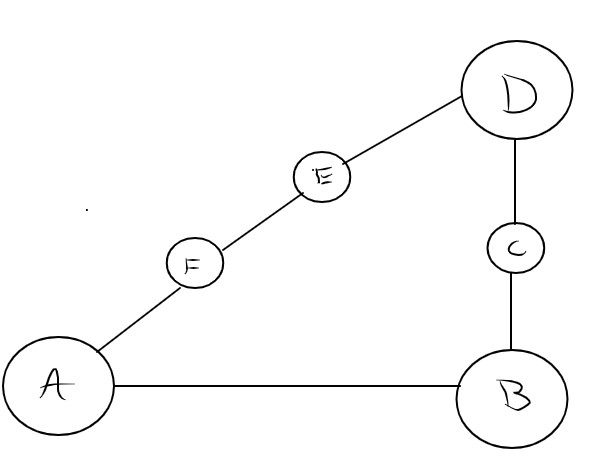
\includegraphics[scale=0.5]{z9top}	
\end{center}

\noindent
Następuje awaria łącza między \(A\) i \(B\). Dowiadują się one o tym i natychmiast zaczynają zalewać sieć informując o zmienionej kolejności. Załóżmy że przesłanie pakietu łączem kosztuje jedną jednostkę czasu. Po upływie jednej takiej jednostki będą routery, do których dotarła informacja o awarii (\(F\) i \(C\)) oraz routery, które wciąż widzą topologię taką jaka była przed awarią (\(D\) i \(E\)).

Przed awarią, pakiety wysyłane do \(A\) byłyby przekazywane przez router \(D\) do routera \(C\) i w tym momencie dalej tak będzie, bo nie wie on jeszcze o awarii. Natomiast \(C\) już się o niej dowiedział, zatem zacznie wysyłać pakiety kierowane do \(A\) przez \(D\). Mamy cykl.

\begin{center}
	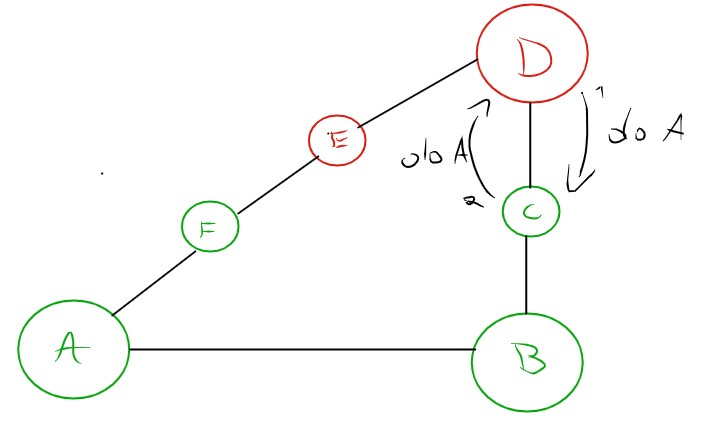
\includegraphics[scale=0.5]{z9cycle}	
\end{center}

\vskip 0.2cm
\noindent
\textbf{Zadanie 10} Załóżmy, że sieć składa się z łączy jednokierunkowych (tj. topologia sieci jest grafem skierowanym) i nie zawiera cykli. Rozważmy niekontrolowany algorytm ,,zalewający'' sieć jakimś komunikatem: komunikat zostaje wysłany początkowo przez pewien router; każdy router, który dostanie dany komunikat przysyła go dalej wszystkimi wychodzącymi z niego krawędziami. Pokaż, że istnieją takie sieci z \(n\) routerami, w których przesyłanie informacji zakończy się po czasie \(2^{\Omega(n)}\). Zakładamy, że przez jedno łącze można przesłać tylko jeden komunikat naraz, a przesłanie go trwa jednostkę czasu.
\vskip 0.2cm

\noindent
\textbf{Rozwiązanie:} Konstruujemy graf sieci w następujący sposób:

\begin{itemize}
	\item Ustalamy porządek na wierzchołkach. Nazywamy je (\(V_1, V_2, ..., V_n\)). \(V_1\) to router który wysyła pierwszy pakiet.
	\item Każdy wierzchołek od \(V_1\) do \(V_{n-2}\) łączymy krawędzią wychodzącą z każdym wierzchołkiem o większym indeksie.
	\item Dodajemy krawędź z \(V_{n-1}\) do \(V_n\).
\end{itemize}

\noindent
Przykład dla \(n=5\):

\begin{center}
	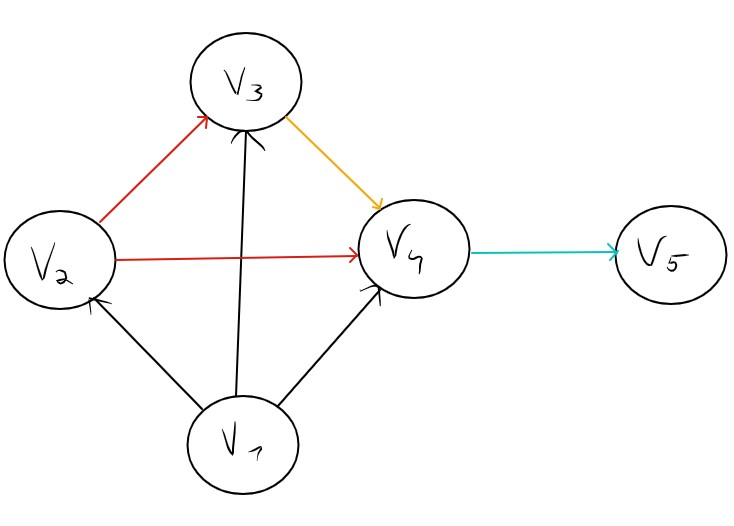
\includegraphics[scale=0.5]{z10exe}	
\end{center}

\noindent
W takim grafie nie będzie cykli, gdyż kolejne wierzchołki w dowolnej ścieżce mają indeksy w ściśle rosnącej kolejności.

Pokażemy, że w takim grafie wierzchołek \(V_i \in \{V_i,...,V_{n-1}\} \), \( 1 \leq i \leq n-1\) będzie miał do wysłania aż \(2^{i-1}\) pakietów, co będzie również oznaczać, że w szczególności \(V_{n-1}\) musi wysłać \(2^{n-1}\) pakietów do \(V_n\), zatem potrzebne jest co najmniej tyle jednostek czasu. Można to zrobić indukcyjnie po wielkości sieci składającej się z routerów \(V_1, V_2, ..., V_{n-1}\). Liczność tej sieci oznaczymy \(w\).

Dla \(w=1\) jest w niej jeden router \(V_1\) i jest on tym startowym, zatem wyśle dokładnie \(1 = 2^{1 - 1}\) pakietów.

Załóżmy, że tak jest dla dowolnego \(k \in \mathbb{N}\), \( 1 \leq k \leq w\). Pokażemy że zachodzi to też dla \(w+1\). Zauważmy, że graf składający się z wierzchołków \(V_1, V_2, ..., V_{w}\) to mniejszy  graf dla którego zachodzi nasze założenie indukcyjne. Wierzchołek \(V_{w+1}\) ma krawędź wchodzącą od każdego wierzchołka od mniejszym indeksie, czyli otrzyma od nich (zgodnie z założeniem indukcyjnym):
\[
	2^0 + 2^1 + ... + 2^{w-1} = 2^{w}
\]
pakietów, które będzie musiał przesłać dalej. Co kończy dowód.

\end{document}
